\documentclass[tikz,border=2pt]{standalone}
\usepackage{xcolor}
\usepackage{pgfplots}
\usetikzlibrary{arrows.meta}

\pgfplotsset{compat=1.16}
\pgfplotsset{
  singlebarlegend/.style={
    legend image code/.code={
      \draw[##1] (0cm,-0.08cm) rectangle (0.25cm,0.08cm);
    }
  }
}

\definecolor{paperBlue}{RGB}{55,96,146}
\definecolor{paperTeal}{RGB}{74,135,126}
\definecolor{paperGold}{RGB}{190,137,48}
\definecolor{paperRed}{RGB}{164,78,76}
\definecolor{paperGray}{RGB}{92,92,92}

\begin{document}
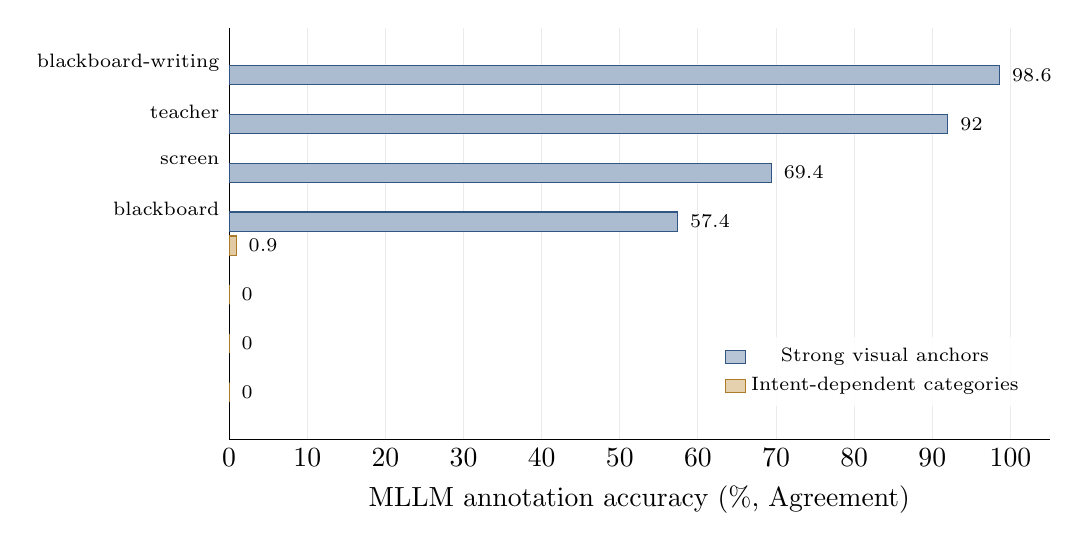
\begin{tikzpicture}
\begin{axis}[
  width=12.0cm,
  height=6.8cm,
  xbar,
  bar width=7pt,
  xmin=0, xmax=105,
  xlabel={MLLM annotation accuracy (\%, Agreement)},
  symbolic y coords={on-stage interaction,guide,answer,stand,blackboard,screen,teacher,blackboard-writing},
  ytick=data,
  y tick label style={font=\scriptsize},
  axis x line*=bottom,
  axis y line*=left,
  xmajorgrids=true,
  grid style={draw=black!8},
  major tick length=0pt,
  singlebarlegend,
  legend style={at={(0.98,0.08)}, anchor=south east, font=\scriptsize,
                draw=none, fill=white, fill opacity=0.85, text opacity=1},
  nodes near coords={\pgfmathprintnumber[fixed,precision=1]{\pgfplotspointmeta}},
  point meta=x,
  nodes near coords style={font=\scriptsize, anchor=west, xshift=1pt},
]
\addplot[fill=paperBlue!42, draw=paperBlue!90!black] coordinates {
  (98.6,blackboard-writing)
  (92.0,teacher)
  (69.4,screen)
  (57.4,blackboard)
};
\addplot[fill=paperGold!45, draw=paperGold!90!black] coordinates {
  (0.9,stand)
  (0.0,answer)
  (0.0,guide)
  (0.0,on-stage interaction)
};
\legend{Strong visual anchors, Intent-dependent categories}
\end{axis}
\end{tikzpicture}
\end{document}